\documentclass[a4paper,11pt]{article}
\usepackage{graphicx}
\usepackage{wrapfig}
\usepackage[a4paper, inner=3cm, outer=3cm, top=3cm, bottom=3cm, offset=0cm]{geometry}
\author{Kenneth Cross : 009200022
        \\Brendan Donahue : 007597252
        \\Mason Itkin : 007777029
        \\CMPE 130 : Tue - Thur : 1500
        \\San Jose State University}
\title{\textbf{Scheduling Algorithm}}
\date{\today}

\begin{document}
\pagenumbering{gobble}
\maketitle
\newpage
\tableofcontents
\newpage
\pagenumbering{arabic}
\setcounter{page}{1}

\section{Executive Summary}

The scheduler algorithm is a program that allows businesses to input employee availability and output a weekly schedule.  The input into the algorithm is a simple spreadsheet including each employee and their availability depending on the day of the week.  Once the entire staff is entered into the computer it will match the employees open availability with open shifts on the schedule.   The program outputs the weekly schedule on a clean color coated spread sheet showing each employees shifts for the week.  While the program does work flawlessly, extra time would have allowed us to add more complexity to better aid the user in creating a more fair and balanced schedule. 

\newpage

\section{Introduction} 
 

While shift scheduling algorithms have been accomplished before they are still not widely used.  This is due to the high cost of the software and the complexity of use.  The aim of this project was to simplify the algorithm using a different programming language, R to make the program easier and cleaner while still reaching the desired effect.  R is an uncommon programing language but it was used for this project because of its simple graphic output and statistical analysis capabilities.  This language allows for the program to easily analyze the input availabilities and find corresponding shifts for each employee based on previously determined shift times.  The desired goal was to have a program with a simple input that could be used by anyone while still achieving a working schedule that can be easily printed or posted online.

\section{Background and Objectives}

Shift Scheduling programs allow users to input multiple availabilities and receive an output of the schedule showing which employees are working which shifts.  These programs already exist but are not widely used.  Great scheduling programs have come out, but they are not free and in some cases can cost over \$1,000 a year.  While these large online based scheduling programs have a complete graphic user interface, they can become over complicated and over priced for smaller companies.

The main objective of this project was to program a simplified scheduling algorithms that was easy to use for smaller companies.  This lead to starting a new scheduling from scratch and just coding what was needed.  Using the programming language R was never an objective but was almost a necessity when coding this kind of program.  Our algorithm allows the user to determine shift times, shift lengths, and employee availability to allocate each employee to the open shift that best fits their availability.  This is an extremely simplistic version of a shift scheduling program but the main algorithm works flawlessly and can be easily edited to add other parameters or modules. 

 Our development time table for this project wasn’t perfect, some earlier objectives for this program were dropped to make time for new objectives. While initially the program was planned to have more input parameters such as priority and position the time spent coding this was exchanged to create a simplified output of the already working program.  The option for scheduling priority would have been a good feature option but the more complex code would have taken time away from coding an HTML based output schedule that can easily be printed or posted online. Ultimately, we felt that the focus on a clean and concise workflow with HTML output was more important for the initial release version of our algorithm.

\section{Approach/Methodology}

\textit{R} was chosen because it is easy to use and create rapid prototypes due to its ease of use while handling data. The algorithm was designed uniquely where the final output does not make use of dynamic programming capabilities. It is not a recursive process that uses memorization, but instead is an iterative process. The reason for this design and lack of dynamic programming at the moment is due to the approach used to represent data, which is a table of values, where the algorithm itself runs through a directed cyclic graphing process. In order to utilize dynamic programming, our algorithmic structure would need to be represented as a directed acyclic graph, in a recursive process that utilizes memorization. 

\begin{wrapfigure}{r}{4.5cm}
    \includegraphics[height=10cm]{graph.eps}
    \caption{\small Algorithm Digraph}
\end{wrapfigure}

The actual algorithmic flow of data variables and processes can be viewed in the diagram. It essentially takes a \textit{position-centric} view. To give variability to datasets, randomization of person order when all the data is first initialized, was done. Each run of the entire program causes the output to change. This is desirable for a few reasons; firstly, the appearance of favorability is minimized, since each run takes the person's order in the table into account while scheduling; secondly, the output most likely changes through each run, which makes scheduling more flexible due to user errors in availability lists. Randomization can also be used as an optimization test to look for corner cases, and to find methods to optimize schedules for human desirability rather than pragmatic ease. 

After the data is randomized, the first person in the table is initialized. Next, it goes to check and see if the position that the person is going to be scheduled for is already filled. Given that the position is not filled, it will check to see if the person is available on that day of the week. If the person can indeed work on that day, whether or not the person can perform that type of job is checked. Once it is known that they can, the row of positions is compared to see whether or not it is full. If it is, the next day is filled out until there are no more \textit{next days} columns. When that field is exhausted, the schedule is completed. 

The scheduling algorithm outputs the completed schedule in a professionally formatted HTML table through the use of a custom created formatting tool. When the scheduling part of the algorithm is finished, the completed schedule is outputted into a comma separated values (CSV) file with the use of the R function \textit{write.csv}. This newly created CSV file is then given to a custom created command line tool aptly named CsvToHtml. CsvToHtml is a lightweight formatting algorithm that we created to take individual elements of the CSV file and input them into a presentable HTML table. CsvToHtml works by first writing some preformatted HTML and CSS style code to provide a set of formatting variables for the HTML language. Next, elements are read sequentially and given state flags to separate headers from regular elements and to give certain values special formatting. Finally some small preformatted HTML code is appended to the end, creating a properly formatted HTML file. HTML was chosen because it is a highly customizable and widely supported file type. Users can quickly print the html schedule to post in the workplace or easily integrate it into an existing website or an online employee portal.
 
\section{Findings and Analysis}

Since the pragmatic flow of the algorithm still runs through a directed cyclic graph process, the future versions of it plan to be reworked in order for it to run through an acyclic process. This can be easily achieved without reworking of the data structure, although data representation changes can still occur if it were able to simplify algorithmic complexity and improve performance at runtime. Because the application of the algorithm itself requires small data-sets, actual operational complexity is of minimal importance, as the scheduling operations should try to increase actual physical scheduling outcomes for humans. In the future, a person-centric algorithmic order is desirable because the outcome in which people are happy is often more important than the outcome in which positions are filled.

\section{Conclusion and Recommendations}
A shift scheduling program utilizes all abilities in programming. While the shift scheduling algorithm was the main focus of the project, a lot of other coding was needed to make it viable for use. The algorithm needed a simple input that would be easy to use by a store manager and an output that is easy to read by the employees. Programming the input and output of the program took away from adding more complexity to the algorithm. This time crunch is what leads to most of the recommendations. 

The best way to improve this program would be to add more complexity to the algorithm that relates to human desirability factors. Firstly, the ability for the algorithm to take priority into account would be useful. Most jobs schedule those who are higher up or who have worked with the company the longest first. This allows those who have higher priority to get more shifts and better time slots. Adding this functionality to the program would have been easy since the main algorithm was done but reformatting the input and the algorithm was not within the time constraint.  Along the same lines as priority is shift preference, it would have also added an important function to the program.  Programming in an extra variable that shows employee preference towards day or night shifts would have helped the employees get a better schedule.  Again this was planned but not completed due to the time constraints.  The program worked great and output a correct schedule every time but could have had more functionality to make a better schedule. 

\end{document}
